\documentclass[letterpaper,12pt,fleqn]{article}
\usepackage{matharticle}
\usepackage{tikz}
\usepackage{graphicx}
\usepackage{siunitx}
\pagestyle{empty}
\newcommand{\e}{\varepsilon}
\begin{document}

\section*{Problems The Need Calculus}

We have made the statement that everything in real number algebra can be performed using definitions and theorems
based upon the ten axioms, the axioms of equality, and the substitution principle.  But there are some questions
about functions that cannot be easily answered with these basic algebra techniques:
\begin{enumerate}[left=0pt]
\item Is a function continuous?
  
  Up until now we have been doing this visually, looking for holes, jumps, and breaks:

  \begin{minipage}{2in}
    \begin{center}
      \begin{tikzpicture}[scale=0.75]
        \node (h) [draw,circle,inner sep=0pt,minimum size=5pt] at (1,1) {};
        \draw [thick] (-3,0) -- (3,0);
        \draw [thick] (0,-3) -- (0,3);
        \draw (-3,-1) .. controls (-2,3) and (0,0) .. (h) .. controls (1.5,1.7) .. (2,3);
      \end{tikzpicture}

      HOLE
    \end{center}
  \end{minipage}
  \begin{minipage}{2in}
    \begin{center}
      \begin{tikzpicture}[scale=0.75]
        \node (h) [draw,circle,inner sep=0pt,minimum size=5pt] at (0,1) {};
        \node [draw,circle,fill,inner sep=0pt,minimum size=5pt] at (0,0) {};
        \draw [thick] (-3,0) -- (3,0);
        \draw [thick] (0,-3) -- (0,3);
        \draw (-2,3) to (h) to (2,3);
      \end{tikzpicture}

      JUMP
    \end{center}
  \end{minipage}
  \begin{minipage}{2in}
    \begin{center}
      \begin{tikzpicture}[scale=0.75]
        \draw [thick] (-3,0) -- (3,0);
        \draw [thick] (0,-3) -- (0,3);
        \draw [domain=-3:-0.35] plot({\x},{1/\x});
        \draw [domain=0.35:3] plot({\x},{1/\x});
      \end{tikzpicture}

      BREAK
    \end{center}
  \end{minipage}

\item What is the (instantaneous) rate of change of a function at a point?

  Up until now all we can do is make an estimate that we call the \emph{average} rate of change around a point
  based on the slope of a chord drawn between two selected points:

  \begin{center}
    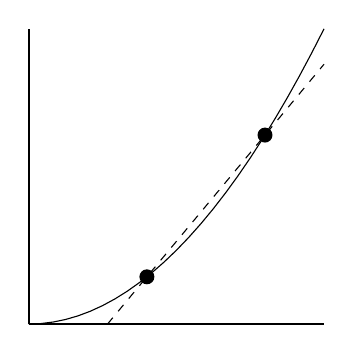
\begin{tikzpicture}[scale=0.75]
        \draw [thick] (0,0) -- (5,0);
        \draw [thick] (0,0) -- (0,5);
        \draw [domain=0:5] plot({\x},{(\x)^2/5});
        \node (a) [draw,circle,fill,inner sep=0pt,minimum size=5pt] at (2,0.8) {};
        \node (b) [draw,circle,fill,inner sep=0pt,minimum size=5pt] at (4,3.2) {};
        \draw [dashed] ({4/3},{0}) to (5,{22/5});
    \end{tikzpicture}
  \end{center}

  But this has the drawback of not being exact and the fact that the function can do weird stuff in between the two
  selected points.

\item Where are the maxima (peaks) and minima (valleys) of a function?

  Up until now we have been plotting the function on a graphing calculator and using the min/max operations:

  \begin{center}
    \includegraphics[scale=0.65]{min.png}
  \end{center}

  \bigskip

\item How do we calculate total amounts when the rate of change is not constant?

  Recall constrant rate of change problems like:
  \[distance=rate\times time\]
  When the rate and time are constant values, then we can just multiply them to obtain the total distance.  For
  example, if a car is traveling at \SI{60}{mph} and travels for \SI{2}{hours}, we can calculate the total distance
  traveled by:
  \[\SI{60}{miles/hour}\cdot\SI{2}{hours}=\SI{120}{miles}\]
  Geometrically, we are calculating the area of the rectangle under the constant rate-of-change curve:

  \begin{center}
    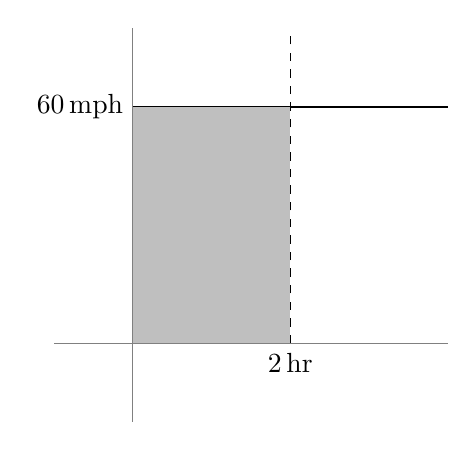
\begin{tikzpicture}
      \draw [help lines] (-1,0) -- (4,0);
      \draw [help lines] (0,-1) -- (0,4);
      \draw (0,3) -- (4,3);
      \node [left] at (0,3) {\SI{60}{mph}};
      \draw [dashed] (2,0) -- (2,4);
      \node [below] at (2,0) {\SI{2}{hr}};
      \fill [fill=white!75!black] (0,0) rectangle (2,3);
    \end{tikzpicture}
  \end{center}

  But what happens when the rate-of-change is a non-constant function of time?

  \begin{center}
    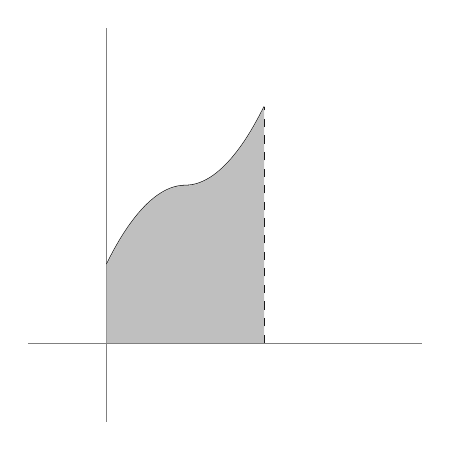
\begin{tikzpicture}
      \draw [help lines] (-1,0) -- (4,0);
      \draw [help lines] (0,-1) -- (0,4);
      \draw [dashed] (2,0) -- (2,3);
      \draw (2,3) parabola bend (1,2) (0,1);
      \fill [fill=white!75!black] (0,0) -- (2,0) -- (2,3) parabola bend (1,2) (0,1) -- cycle;
    \end{tikzpicture}
  \end{center}

  It turns out that the total is still the area under the curve; however, there is no simple geometric formula
  for calculating that area.
\end{enumerate}

\bigskip

To answer these questions we need a new concept: \emph{arbitrarily close}.  Our strategy is going to be to look at
\emph{arbitrarily small} intervals around a point and to see how the function is behaving in that interval.  This
will allow us to make determinations about how the function behaves at the point in question as we get arbitrarily
close to that point.

\end{document}
